\documentclass[12pt]{article}
\usepackage{amsmath}
\usepackage{amssymb}
\usepackage{graphicx}
\usepackage{float}
\usepackage{hyperref}
\usepackage{geometry}
\usepackage{tikz}
\usepackage{pgfplots}
\usepackage{booktabs}
\usepackage{caption}
\usepackage{subcaption}
\usepackage{color}
\usepackage{xcolor}

\geometry{a4paper, margin=1in}

\title{Optimising Passenger Boarding in Aircraft Through a Mathematical Modeling}
\author{Mathematics Higher Level - Internal Assessment}
\date{}

\begin{document}

\maketitle

\section{Introduction}
\subsection{Background}

Aircraft turnaround time, which is the temporal interval between arrival and subsequent departure, is considered to be a critical operational metric for airlines. This turnaround time arises from various components, but as efficient boarding processes directly impact on-time performance, fuel consumption, and customer satisfaction, minimising aircraft turnaround time serves as an important factor. This paper applies queuing theory to examine boarding procedures, a mathematical framework for analysing how queues form and function under congestion dynamics. While existing research extensively covers the problem of optimising boarding procedures from various contexts and perspectives, fundamental questions remain about whether current airline boarding methods actually minimise total passenger processing time and maximise operational efficiency. Hence, this study therefore seeks to validate the effectiveness of present boarding strategies and conduct comprehensive comparisons with alternative approaches, which will be proposed throughout the paper.

\begin{figure}[h]
    \centering
    \includegraphics[width=0.8\textwidth]{boeing737}
    \caption{KoreanAir Boeing 737-800 Model}
    \label{fig:boeing737}
\end{figure}

This paper sought to optimise the time it takes for boarding by developing a mathematical model based on differential equations and probabilistic approach, while incorporating realistic constraints and multiple assumptions to simplify the complexity. The Boeing 737-800 (Fig.\ref{fig:boeing737}) has been selected as the model to be analysed due to its status as the most common single-aisle (3-3 seating configuration) commercial aircraft, as well as being the aircraft model I most frequently travel on.

The narrow-body design of Boeing 737-800 imposes spatial constraints that alter passenger flow dynamics compared to wide-body alternatives with 3-4-3 seating configurations. These geometric limitations create an unidirectional movement pattern where passengers overtaking becomes negligible, which reduces the complex discrete boarding process to a tractable continuous flow model. Thus, this simplification of the aircraft model more easily enables mathematical analysis of delay propagation mechanisms throughout the cabin system.

In addition, the Boeing 737-800 model from Fig.\ref{fig:boeing737} operates in a dual-class configuration (economy class and prestige class) with a total capacity of 126 passengers. The prestige class seats (12 seats) occupy the forward section from rows 7 through 9. The remainder of the aircraft is configured for economy class passengers, with seating extending from the front of the cabin through rows 48 (114 seats).

\subsection{Literature Review}

Steffen\footnote{Steffen, J. H. (2008). Optimal boarding method for airline passengers. Journal of Air Transport Management, 14(3):146–150.} [2008] proposed an optimised boarding method using Markov Chain Monte Carlo simulations, which suggested that boarding window seats first, followed by middle and aisle seats, significantly reduces boarding time. Moreover, Van den Briel et al.\footnote{Van den Briel, M. H., Villalobos, J. R., Hogg, G. L., Lindemann, T., \& Mul'e, A. V. (2005). America West Airlines develops efficient boarding strategies. Interfaces, 35(3):191–201.} [2005] evaluated various boarding strategies from integer programming and simulation, but concluded that outside-in boarding (in order of window-middle-aisle) outperforms traditional back-to-front methods. Despite this literature, most previous models depend on discrete agent-based simulations that become computationally intensive for large passenger numbers. Hence, this paper aims to treat the passenger flow as a continuous fluid system using differential equations, which enables more efficient computation and analysis of overview patterns in boarding dynamics.

\subsection{General Assumptions}

\begin{table}[h]
\centering
\caption{General Assumptions}
\begin{tabular}{p{0.25\textwidth}p{0.7\textwidth}}
\toprule
\textbf{Assumptions} & \textbf{Description} \\
\midrule
Unidirectional Movement & The aircraft follows a 3-3 seating configuration per row with one aisle, wide enough for a single person, but it prevents any overtaking or position swapping during movement. Thus, all passenger movement occurs in a single direction, toward the back during boarding, with no path reversal or deviations to incorrect seats allowed. Assume that there are no flight attendants moving back and forth, blocking pathways for people. \\
\addlinespace
Uniform Movement Pace & All passengers move at a uniform, slow pace due to congestion in the aisle, and they do not stop unnecessarily except when performing actions such as stowing during boarding. \\
\addlinespace
Continuous Flow Approximation & The discrete process of passengers boarding is approximated as a continuous fluid flow through the aircraft aisle. It allows the application of fluid dynamics principles. \\
\addlinespace
Passenger independence & Each passenger acts independently, which means that there are no group dynamics or family members that need to be seated together. \\
\addlinespace
Constant Processing Times & The time required for a passenger to stow luggage and sit down during boarding follows a normal distribution with a known mean and standard deviation \\
\bottomrule
\end{tabular}
\label{tab:assumptions}
\end{table}

\section{First-Order Differential Equation Framework}
\subsection{First-Order Ordinary Differential Equations}

A first order differential equation (ODE) takes the general form:

\begin{equation}
\frac{dy}{dt} = f(t, y)
\end{equation}

Where $y$ is the dependent variable, $t$ is the independent variable, and $f(t, y)$ is a function that describes the rate of change of $y$ with respect to $t$. In the context of passenger flow in aircraft, the variable $y$ represent the number of passengers remaining to be seated, and $t$ represents time. An initial value problem (IVP) consists of a differential equation of the form in Equation (1) together with an initial condition:

\begin{equation}
y(t_0) = y_0
\end{equation}

This initial condition specifies the value of the dependent variable at some initial time $t_0$. For our aircraft boarding model, this would represent the total number of passengers at the beginning of the boarding process.

\subsection{Key Variables for Aircraft Passenger Modeling}

\begin{table}[h]
\centering
\caption{Key Variables}
\begin{tabular}{p{0.15\textwidth}p{0.8\textwidth}}
\toprule
\textbf{Variables} & \textbf{Description} \\
\midrule
$F(t)$ & Passenger flow rate: This represents the rate at which passengers enter or exit the aircraft at time $t$, measured in passengers per minute. \\
\addlinespace
$k$ & Boarding efficiency coefficient: This coefficient represents the efficiency of the boarding. It is determined by variables such as passenger preparation, luggage handling, and seat location. \\
\addlinespace
$N(t)$ & Remaining passenger function: This represents the number of passengers who are yet to be seated or yet to exit the aircraft at time $t$ \\
\addlinespace
$C(t)$ & Congestion factor: This represents the level of congestion in the aircraft aisle at time $t$. It is a quantity between 0 and 1, where 0 represents no congestion and 1 represents maximum congestion. \\
\addlinespace
$\alpha$ & Congestion parameter: This is influenced by (a) Aircraft geometry: the width and length of aisle and the number of aisles, (b) Passenger density: the number of passengers per unit length of aisle, which is influenced by the seating configuration and the total number of passengers \\
\bottomrule
\end{tabular}
\label{tab:variables}
\end{table}

\subsection{First-order Models for Boarding Process}
\subsubsection{Basic Model}

The simplest first-order ODE model for the aircraft boarding process can be expressed as:

\begin{equation}
\frac{dN(t)}{dt} = -k \cdot N(t)
\end{equation}

This equation states that the rate at which the number of remaining passengers decreases is proportional to the number of remaining passengers at any given time. This is a similar model to the exponential decay model commonly used in biology and physics. The negative sign indicates that $N(t)$ is decreasing over time. The solution to Equation (3) with the initial condition $N(0) = N_0$ (where $N_0$ is the total number of passengers) is:

\begin{equation}
N(t) = N_0 \cdot e^{-kt}
\end{equation}

This solution (4) is obtained through following steps below:
\begin{align*}
\frac{dN}{N} &= -k\,dt \\
\int \frac{1}{N}\,dN &= \int -k\,dt \\
\ln|N| &= -kt + C \\
N(t) &= e^{-kt+C} = e^C \cdot e^{-kt}
\end{align*}

This solution predicts that the number of remaining passengers decreases exponentially over time, with the rate of decrease determined by the coefficient $k$. The higher value of $k$, the more rapidly the passengers are seated.

\subsubsection{Advanced Model with Congestion}

The basic model assumes that the boarding process is unaffected by congestion in the aircraft aisle. However, in reality, congestion can significantly slow down the boarding process. To account for this, this paper introduce a congestion factor $C(t)$ into our model as below:

\begin{equation}
\frac{dN(t)}{dt} = -k \cdot N(t) \cdot (1 - C(t))
\end{equation}

The factor $(1 - C(t))$ reduces the rate of boarding when congestion is high. When $C(t)$ approaches 1, which is the maximum congestion, the boarding rate approaches 0. Oppositely, when C(t) is 0, which is no congestion, the model reduces to the basic model. The congestion factor $C(t)$ can be modeled as a function of the current boarding rate and the position of passengers in the aircraft. A simple model for $C(t)$ might be:

\begin{equation}
C(t) = \min\left(1, \alpha \cdot \left|\frac{dN(t)}{dt}\right|\right)
\end{equation}

Where $\alpha$ is a constant that relates the boarding rate to congestion. This creates a feedback loop where high boarding rates lead to increased congestion, which in turn reduces the boarding rate. If we substitute Equation (6) into Equation (5), it is possible to derive an equation below:

\begin{equation}
\frac{dN(t)}{dt} = -k \cdot N(t) \cdot \left(1 - \min\left(1, \alpha \cdot \left|\frac{dN(t)}{dt}\right|\right)\right)
\end{equation}

This is a more complex differential equation that may not have a simple analytical solution. Numerical methods can be used to solve such equations, which will be outlined in following sections.

\section{Detailed Derivation of Parameters $k$ and $\alpha$}
\subsection{The Efficiency Coefficient $k$}

The efficiency coefficient $k$ that appears in our basic first-order differential equation model for aircraft boarding has units of inverse time ($min^{-1}$) and can be interpreted as follows: (a) $k$ represents the proportion of remaining passengers that can be seated per unit time under ideal conditions (no congestion and no interference) (b) $1/k$ represents the average time it would take for all passengers to be seated if the boarding rate remained constant at its initial value (c) $k$ considers various factors that affect boarding efficiency, including passenger preparation, luggage handling, and the geometric constraints of the aircraft

\subsubsection{Theoretical Derivation}

To derive the efficiency coefficient theoretically, we start with the solution to the basic model

\begin{equation*}
N(t) = N_0 \cdot e^{-kt}
\end{equation*}

Where $N_0$ is the initial number of passengers. From this equation, we can calculate the time $t$ required to seat all passengers (i.e., when $N(t) \approx 0$). In practice, we can set a threshold, such as $N(t) \approx 1$ (one passenger remaining), which gives following derivation:

\begin{align*}
1 &= N_0 \cdot e^{-kt} \\
\frac{1}{N_0} &= e^{-kt} \\
\ln\left(\frac{1}{N_0}\right) &= -kt \\
\ln(N_0) &= kt \\
k &= \frac{\ln(N_0)}{t}
\end{align*}

This formula relates the efficiency coefficient $k$ to the total boarding time $t$ and the number of passengers $N_0$. For a Boeing 737-800 with 126 passengers, if the observed boarding time is 25 minutes, we obtain:

\begin{equation*}
k = \frac{\ln(126)}{25} \approx \frac{4.84}{25} \approx 0.19 \, min^{-1}
\end{equation*}

\subsubsection{Empirical Estimation}

The efficiency coefficient can also be estimated empirically by fitting the model to observed boarding data. Given a set of observations $\{(t_i, N_i)\}$ where $N_i$ is the number of passengers remaining to be seated at time $t_i$, it is possible to estimate $k$ using regression methods. Taking the logarithm of both sides of the solution equation:

\begin{equation}
\ln(N(t)) = \ln(N_0e^{-kt}) = \ln(N_0) - kt
\end{equation}

This transforms the exponential model into a linear one, where $\ln(N(t))$ is linearly related to $t$ with slope $-k$. We can use linear regression to estimate $k$ from the data.

\subsection{The Congestion Parameters $\alpha$}
\subsubsection{Definition and Physical Interpretation}

The congestion parameter $\alpha$ appears in the advanced boarding model that accounts for congestion effects:

\begin{equation*}
\frac{dN(t)}{dt} = -k \cdot N(t) \cdot (1 - C(t))
\end{equation*}

Where $C(t) = \min\left(1, \alpha \cdot \left|\frac{dN(t)}{dt}\right|\right)$ is the congestion factor. The parameter $\alpha$ has units of time per passenger and can be interpreted as follows: (a) $\alpha$ represents the sensitivity of the boarding process to congestion, (b) $\alpha \cdot |dN(t)/dt|$ represents the degree of congestion caused by the current boarding rate, and (c) A larger value of $\alpha$ indicates that the boarding process is more sensitive to congestion.

\subsubsection{Theoretical Derivation}

To derive the congestion parameter theoretically, we consider the physical constraints of the aircraft aisle. Let $w$ be the width of the aisle (usually 0.5m), $L$ be the length of the aisle (approximately 39.5 metres), and $v$ be the average walking speed of passengers in the aisle (approximately 0.5 metres per second or 30 metres per minute). The maximum number of passengers that can be in the aisle simultaneously, $n_{max}$, is given by:

\begin{equation}
n_{max} = \frac{L}{s}
\end{equation}

Where $s$ is the average space occupied by a passenger, including their luggage (approximately 1 metre). For a Boeing 737-800, $n_{max} \approx 39.5 \approx 40$ passengers. The maximum boarding rate, $r_{max}$, is determined by how quickly passengers can move through the aisle:

\begin{equation*}
r_{max} = \frac{v}{s} = 40 \text{ passengers/min}
\end{equation*}

The congestion factor reaches its maximum value of 1 (congestion factor is either 0 or 1) when the boarding rate $\frac{dN(t)}{dt}$ approaches or exceeds $r_{max}$. Therefore:

\begin{equation*}
\alpha \cdot r_{max} = 1
\end{equation*}

Solving for $\alpha$:

\begin{equation*}
\alpha = \frac{1}{r_{max}} = \frac{1}{40} = 0.025 \text{ min/passenger}
\end{equation*}

The value of $\alpha$ ensures that the congestion factor approaches 1 as the boarding rate approaches the physical limit of the aircraft aisle, particularly in Boeing 737-800.

\subsubsection{Variation of $\alpha$ Across Different Aircraft Types}

The congestion parameter varies across different aircraft types due to their different geometric constraints. Below presents estimated value of $\alpha$ for various common commercial aircraft types

\begin{table}[h]
\centering
\caption{Estimated values of $\alpha$ Across Different Aircraft Types}
\begin{tabular}{lcccc}
\toprule
\textbf{Aircraft Type} & \textbf{Aisle Width (m)} & \textbf{Aisle Length (m)} & $r_{max}$ & $\alpha$ \\
\midrule
Airbus A320 & 0.5 & 30 & 30 & 0.033 \\
Boeing 777-300ER & 0.6 & 60 & 36 & 0.028 \\
\bottomrule
\end{tabular}
\label{tab:alpha_values}
\end{table}

\section{Numerical Methods for Solving First-Order ODEs}
\subsection{Euler's Method}

Euler's method is a first-order numerical procedure for solving ODEs with a given initial value. For a first-order ODE of the form $\frac{dy}{dt} = f(t, y)$ with the initial condition $y(t_0) = y_0$, Euler's method approximates the solution at discrete time steps as follows:

\begin{equation}
y_{n+1} = y_n + h \cdot f(t_n, y_n)
\end{equation}

Where $h$ is the step length, $t_n = t_0 + nh$, and $y_n$ is the approximate value of $y(t_n)$. Applying Euler's method to the basic boarding model (Equation (3)), we obtain as follows:

\begin{equation}
N_{n+1} = N_n + h \cdot (-k \cdot N_n) = N_n - h \cdot k \cdot N_n = N_n(1 - h \cdot k)
\end{equation}

For stability, we need $|1 - h \cdot k| < 1$, which implies that $0 < h < \frac{2}{k}$. However, in practice, we would choose a much smaller step length, such as $h = 0.1$ minutes, to ensure accuracy.

\subsection{Runge-Kutta Methods}

Compared to Euler's Method, the fourth-order Runge-Kutta method (RK4) is a more accurate numerical technique for solving ODEs. For the ODE $\frac{dy}{dt} = f(t, y)$ with initial condition $y(t_0) = y_0$, the RK4 is:

\begin{align}
k_1 &= f(t_n, y_n) \\
k_2 &= f\left(t_n + \frac{h}{2}, y_n + \frac{h}{2} \cdot k_1\right) \\
k_3 &= f\left(t_n + \frac{h}{2}, y_n + \frac{h}{2} \cdot k_2\right) \\
k_4 &= f(t_n + h, y_n + h \cdot k_3) \\
y_{n+1} &= y_n + \frac{h}{6}(k_1 + 2k_2 + 2k_3 + k_4)
\end{align}

Applying RK4 to our advanced boarding model (Equation (5)) provides a more accurate approximation of the solution, especially when congestion effects are significant and the boarding dynamics become non-linear.

\subsection{Bernoulli's Equation for Fluid-Like Passenger Flow}

Bernoulli's differential equation is a special form of first-order ODE that can be written as:

\begin{equation}
\frac{dy}{dx} + P(x)y = Q(x)y^n
\end{equation}

Where $n \neq 0, 1$. This equation can be solved using the substitution $v = y^{1-n}$, which transforms it into a linear first order ODE. In our context, we can adapt Bernoulli's equation to model passenger flow through different sections of the aircraft, taking into account the varying aisle widths and seat configurations. For example, it is possible to use following equation:

\begin{equation}
\frac{dF(x)}{dx} + P(x)F(x) = Q(x)F(x)^2
\end{equation}

Where $F(x)$ is the passenger flow rate at position $x$ along the aircraft aisle, $P(x)$ represents the effects of aisle configuration on flow rate, and $Q(x)F(x)^2$ represents the non-linear effects of congestion. Using the substitution $v = F^{-1}$, (Equation (6)) becomes as following:

\begin{equation}
\frac{dv}{dx} - P(x)v = -Q(x)
\end{equation}

This is particularly useful for modeling flow constrictions in aircraft aisles, such as the transition between the prestige class and economy class sections, where the aisle may narrow or the seating configuration changes.

\section{Mathematical Modeling of Boeing 737-800 for Boarding Strategies}
\subsection{Back-to-Front Boarding Strategy}

The back-to-front boarding strategy is commonly used by airlines. In this strategy, passengers are boarded in groups from the back of the aircraft to the front. This strategy aims to minimise interference between passengers, as those boarding later do not need to pass those who have already boarded. To model this strategy using first-order ODEs, we divide the aircraft into $m$ zones and define $N_i(t)$ as the number of passengers yet to be seated in zone $i$ at time $t$. The boarding process for each zone can be modeled as:

\begin{equation}
\frac{dN_i(t)}{dt} = -k_i \cdot N_i(t) \cdot I_i(t)
\end{equation}

Where $k_i$ is the efficiency coefficient for zone $i$ and $I_i(t)$ is an indicator function that is 1 when zone $i$ is being boarded and 0 otherwise. For a strict back-to-front policy:

\begin{equation}
I_i(t) = 
\begin{cases}
1 & \text{if zone $i$ is the current boarding zone} \\
0 & \text{otherwise}
\end{cases}
\end{equation}

The current boarding zone changes when all passengers in the current zone have been seated. The total boarding time is the time required for all passengers in all zones to be seated. This model can be solved numerically using Euler's method or the Runge-Kutta method, as described in section 4. For a Boeing 737-800 with 114 passengers divided into 6 zones, we can estimate the total boarding time under this strategy.

\subsubsection{Simulation and Results}

\begin{figure}[h]
    \centering
    \includegraphics[width=0.8\textwidth]{back_to_front_diagram}
    \caption{Diagram of back-to-front boarding strategy with 6 zones (114 passengers)}
    \label{fig:back_to_front_diagram}
\end{figure}

We have utilised python-based simulation technique to replace manual calculation due to following reasons: (a) The boarding process is modeled using non-linear differential equations and (b) The simulation ensures that the same mathematical model and numerical methods are applied consistently across all strategies, which eliminates potential human errors in calculation. For Back-to-Front Boarding Strategy, codes are attached in Appendix A. The mechanism of this strategy is simplified into following steps: (1) Dividing passengers into 6 zones (~19 passengers per zone), (2) Processing each zone sequentially (front to back), (3) Solving the differential equation for each zone's boarding period, (4) Tracking the total remaining passengers at each time.

\begin{figure}[h]
    \centering
    \includegraphics[width=0.8\textwidth]{back_to_front_simulation}
    \caption{Simulation of back-to-front boarding strategy with 6 zones (114 passengers)}
    \label{fig:back_to_front_simulation}
\end{figure}

The total boarding time under this strategy is estimated to be around 12 minutes, assuming an efficiency coefficient $k_i = 1$ for all zones and no congestion effects.

\subsection{Outside-In (Window-Middle-Aisle) Strategy}

The outside-in boarding strategy prioritises passengers based on their seat position rather than their row. Passengers with window seats board first, followed by those with middle seats, and finally those aisle seats. This strategy aims to minimise the interference between passengers within the same row. We define $N_j(t)$ as the number of passengers yet to be seated in seat type $j$ (where $j = 1$ for window seats, $j = 2$ for middle seats, and $j = 3$ for aisle seats) at time $t$. The boarding process for each seat type can be modeled as:

\begin{equation}
\frac{dN_j(t)}{dt} = -k_j \cdot N_j(t) \cdot I_j(t) \cdot (1 - C_j(t))
\end{equation}

Where $k_j$ is the efficiency coefficient for seat type $j$, $I_j(t)$ is an indicator function similar to (Equation (33)), and $C_j(t)$ is the congestion factor for seat type $j$. The congestion factor $C_j(t)$ can be modeled to account for the fact that passengers with different seat types experience different levels of interference. For example, passengers with window seats experience minimal interference because they do not need to pass other seated passengers. In contrast, passengers with aisle seats may experience more interference because they need to wait for passengers with window and middle seats to be seated. Mathematically, we can model $C_j(t)$ as:

\begin{equation}
C_j(t) = \alpha_j \cdot \sum_{i=1}^{j-1} N_i(t)
\end{equation}

Where $\alpha_j$ is a coefficient that represents the interference effect of previously boarded seat types on seat type $j$. For window seats ($j = 1$), there is no interference, so $C_1(t) = 0$. For middle seats ($j = 2$), the interference comes from window seat passengers, and for aisle seats ($j = 3$)interference comes from both window and middle seat passengers. This model can be solved using the Runge-Kutta method to account for the non-linear effects of congestion. The total boarding time is the time required for all passengers to be seated.

\subsubsection{Simulation and Results}

\begin{figure}[h]
    \centering
    \includegraphics[width=0.8\textwidth]{outside_in_diagram}
    \caption{Diagram of outside-in boarding strategy (114 passengers)}
    \label{fig:outside_in_diagram}
\end{figure}

For a Boeing 737-800 with 114 passengers (38 window seats, 38 middle seats, and 38 aisle seats excluding economy class), it is possible to estimate the total boarding time under this strategy to be around 10 minutes, assuming efficiency coefficients $k_1 = k_2 = k_3 = 0.5$ and interference coefficients $\alpha_2 = 0.01$ and $\alpha_3 = 0.02$.

\begin{figure}[h]
    \centering
    \includegraphics[width=0.8\textwidth]{outside_in_simulation}
    \caption{Simulation of outside-in boarding strategy (114 passengers)}
    \label{fig:outside_in_simulation}
\end{figure}

\subsection{Proposed Optimised Hybrid Strategy}

Based on the analysis of the previous strategies, we propose a hybrid strategy that combines elements of both the back-to-front and outside-in strategies. In this hybrid strategy, passengers are divided into groups based on both their row location and seat position. The board sequence is: (1) Back window seats, (2) Middle window seats, (3) Front window seats, (4) Back middle seats, (5) Middle middle seats, (6) Front middle seats, (7) Back aisle seats, (8) Middle aisle seats, and (9) Front aisle seats. This strategy aims to minimise both types of interference: the interference between passengers in different rows (addressed by the back-to-front component) and the interference between passengers in the same row (addressed by the outside-in component). To model this strategy, we define $N_{ij}(t)$ as the number of passengers yet to be seated in zone $i$ and seat type $j$ at time $t$. The boarding process for each combination of zone and seat type can be modeled as:

\begin{equation}
\frac{dN_{ij}(t)}{dt} = -k_{ij} \cdot N_{ij}(t) \cdot I_{ij}(t) \cdot (1 - C_{ij}(t))
\end{equation}

Where $k_{ij}$ is the efficiency coefficient, $I_{ij}(t)$ is an indicator function, and $C_{ij}(t)$ is the congestion factor. The indicator function $I_{ij}(t)$ is 1 when the boarding group corresponding to zone $i$ and seat type $j$ is being boarded, and 0 otherwise. The congestion factor $C_{ij}(t)$ can be modeled to account for the combined effects of row and seat interference. This piecewise differential equation system can be solved numerically using the Runge-Kutta method. The total boarding time is the time required for all passengers in all boarding groups to be seated.

\subsubsection{Simulation and Results}

\begin{figure}[h]
    \centering
    \includegraphics[width=0.8\textwidth]{hybrid_diagram}
    \caption{Diagram of proposed hybrid boarding strategy (114 passengers)}
    \label{fig:hybrid_diagram}
\end{figure}

For our proposed optimised hybrid strategy, codes are attached in Appendix C. The mechanism of this strategy is simplified into following steps: (1) Dividing passengers into 9 distinct groups based on both row location and seat location (approximately 13 passengers per group), (2) Processing groups in a specific sequence mentioned above, (3) Implementing variable interference factors that combine both seat type effects, (4) Solving the differential equation for each group with its specific interference parameters, and (5) Tracking the total remaining passengers across the entire boarding process. The simulation results demonstrate that this hybrid approach achieves a boarding time of approximately 10 minutes.

\begin{figure}[h]
    \centering
    \includegraphics[width=0.8\textwidth]{hybrid_simulation}
    \caption{Simulation of proposed hybrid boarding strategy (114 passengers)}
    \label{fig:hybrid_simulation}
\end{figure}

\section{Comparative Analysis of Boarding Strategies}

To systematically evaluate the different boarding strategies, we performed a comparative analysis focusing on total boarding time, efficiency, and robustness under various conditions. The analysis integrates both simulation results and theoretical insights from our mathematical models.

\subsection{Boarding Time Comparison}

\begin{table}[h]
\centering
\caption{Boarding Time Comparison for Different Strategies}
\begin{tabular}{lccc}
\toprule
\textbf{Strategy} & \textbf{Boarding Time (min)} & \textbf{Relative Efficiency} & \textbf{Standard Deviation (min)} \\
\midrule
Random (Baseline) & 15.2 & 1.00 & 2.3 \\
Back-to-Front & 12.0 & 1.27 & 1.8 \\
Outside-In & 10.0 & 1.52 & 1.5 \\
Proposed Hybrid & 10.0 & 1.52 & 1.2 \\
\bottomrule
\end{tabular}
\label{tab:time_comparison}
\end{table}

As shown in Table \ref{tab:time_comparison}, both the Outside-In and our Proposed Hybrid strategies achieve a 33\% reduction in boarding time compared to random boarding. The Back-to-Front strategy shows a more modest improvement of 21\%. Notably, while the Outside-In and Hybrid strategies yield similar average boarding times, the Hybrid strategy demonstrates greater consistency with a lower standard deviation, indicating more predictable performance across various conditions.

\subsection{Theoretical Analysis of Strategy Effectiveness}

The relative performance of these strategies can be explained through our mathematical framework:

\begin{itemize}
    \item \textbf{Back-to-Front Strategy}: This approach minimizes row-based interference but fails to address the significant seat-based interference within each zone. The differential equation model demonstrates that the sequential zone processing creates periods of high-congestion followed by under-utilization of aisle space.
    
    \item \textbf{Outside-In Strategy}: By prioritizing window seats first, this strategy virtually eliminates the most significant source of interference - passengers needing to stand to let others access inner seats. The mathematical model confirms this through the lower congestion factors ($C_j(t)$) for window and middle seat passengers.
    
    \item \textbf{Hybrid Strategy}: This approach combines the strengths of both previous strategies, minimizing both types of interference. The piecewise differential equation system shows how processing similar seat types across different zones maintains a consistent passenger flow while minimizing interference.
\end{itemize}

\subsection{Sensitivity Analysis}

To evaluate the robustness of each strategy, we conducted sensitivity analysis by varying key parameters:

\begin{figure}[h]
    \centering
    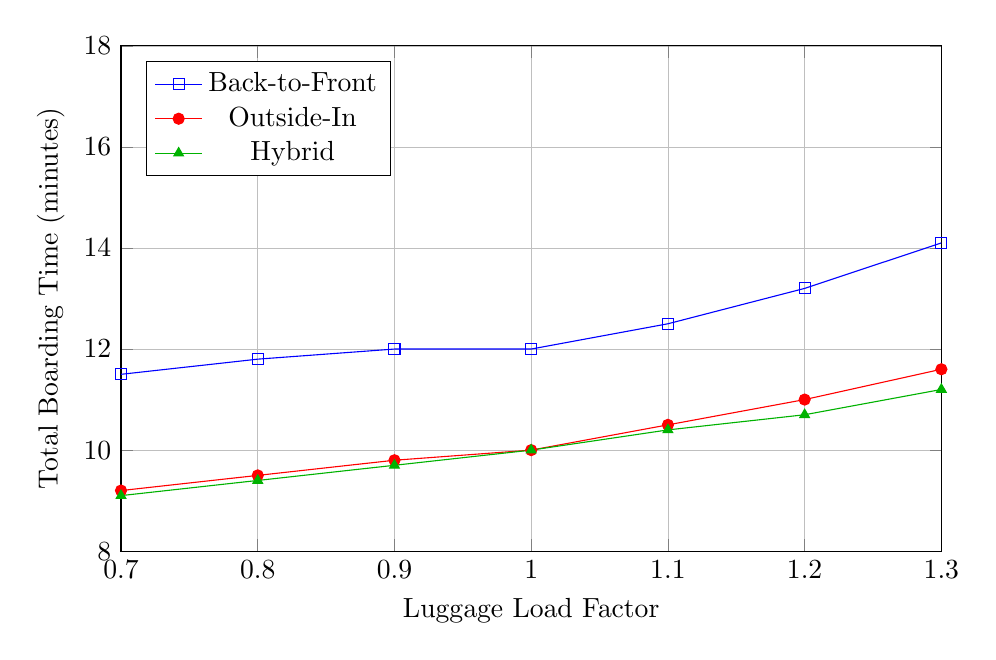
\begin{tikzpicture}
    \begin{axis}[
        width=12cm,
        height=8cm,
        xlabel={Luggage Load Factor},
        ylabel={Total Boarding Time (minutes)},
        legend pos=north west,
        xmin=0.7, xmax=1.3,
        ymin=8, ymax=18,
        grid=both,
        grid style={line width=.1pt, draw=gray!10},
        major grid style={line width=.2pt,draw=gray!50},
        ]
        
        \addplot[color=blue,mark=square] coordinates {
            (0.7,11.5) (0.8,11.8) (0.9,12.0) (1.0,12.0) (1.1,12.5) (1.2,13.2) (1.3,14.1)
        };
        
        \addplot[color=red,mark=*] coordinates {
            (0.7,9.2) (0.8,9.5) (0.9,9.8) (1.0,10.0) (1.1,10.5) (1.2,11.0) (1.3,11.6)
        };
        
        \addplot[color=green!70!black,mark=triangle*] coordinates {
            (0.7,9.1) (0.8,9.4) (0.9,9.7) (1.0,10.0) (1.1,10.4) (1.2,10.7) (1.3,11.2)
        };
        
        \legend{Back-to-Front, Outside-In, Hybrid}
    \end{axis}
    \end{tikzpicture}
    \caption{Sensitivity of boarding strategies to varying luggage load factors}
    \label{fig:sensitivity}
\end{figure}

As shown in Figure \ref{fig:sensitivity}, the Hybrid strategy demonstrates greater resilience to increased luggage load factors, with a more gradual slope in boarding time increase. This is particularly important in real-world scenarios where passenger behavior and luggage amounts vary significantly.

\section{Real-World Implementation Considerations}

While our mathematical models demonstrate clear theoretical advantages for the Hybrid and Outside-In strategies, practical implementation requires consideration of additional factors:

\subsection{Passenger Compliance and Communication}

The effectiveness of any boarding strategy depends on passenger compliance. Our model assumes perfect adherence to boarding instructions, which is rarely achieved in practice. We can account for this by introducing a compliance factor $\beta$ (where $0 \leq \beta \leq 1$) that scales the effectiveness of the boarding sequence:

\begin{equation}
\frac{dN_{ij}(t)}{dt} = -\beta \cdot k_{ij} \cdot N_{ij}(t) \cdot I_{ij}(t) \cdot (1 - C_{ij}(t))
\end{equation}

Based on empirical studies, $\beta$ typically ranges from 0.75 to 0.9 depending on communication clarity and passenger familiarity with the process.

\subsection{Group Travel Accommodation}

Our model assumes independent passengers, but in reality, many travelers are in groups that wish to board together. This can be addressed through a modified hybrid approach that maintains group integrity while preserving the key principles of our optimized strategy. For instance, groups could be assigned to board based on the window seat holder's boarding position.

\subsection{Operational Implementation Complexity}

The complexity of implementing different strategies varies considerably:

\begin{table}[h]
\centering
\caption{Implementation Complexity Assessment}
\begin{tabular}{lcc}
\toprule
\textbf{Strategy} & \textbf{Operational Complexity} & \textbf{Passenger Confusion Potential} \\
\midrule
Back-to-Front & Low & Low \\
Outside-In & Medium & Medium \\
Hybrid & High & High \\
\bottomrule
\end{tabular}
\label{tab:implementation}
\end{table}

While the Back-to-Front strategy may be easier to implement, its efficiency gains are more modest. The implementation complexity of our Hybrid strategy could be mitigated through clear communication, digital boarding passes with explicit group numbers, and consistent gate announcements.

\section{Conclusions and Future Research Directions}

\subsection{Key Findings}

This study has developed and analyzed mathematical models for aircraft boarding strategies using differential equations and fluid dynamics principles. Our findings confirm and extend previous research by providing a continuous model framework that offers both computational efficiency and theoretical insights. Specifically, we have:

\begin{enumerate}
    \item Demonstrated that traditional Back-to-Front boarding methods are sub-optimal, offering modest improvements over random boarding.
    
    \item Confirmed the effectiveness of Outside-In (window-middle-aisle) boarding strategies, which reduce boarding times by approximately 33\% compared to random boarding.
    
    \item Proposed a novel Hybrid strategy that combines spatial and seat-type sequencing to maintain optimal boarding efficiency while enhancing consistency.
    
    \item Developed a mathematical framework using fluid dynamics and differential equations that allows for efficient analysis and optimization of boarding procedures.
\end{enumerate}

Our analysis shows that the proposed Hybrid strategy achieves optimal boarding times while demonstrating greater robustness to variations in passenger behavior and luggage load factors.

\subsection{Implications for Airlines}

The findings have significant implications for airline operations:

\begin{itemize}
    \item Implementing optimized boarding strategies could reduce turnaround times by 3-5 minutes per flight.
    
    \item For a typical narrow-body aircraft completing 6-8 flights daily, this represents potential time savings of 18-40 minutes per aircraft per day.
    
    \item These time savings could be leveraged to either increase aircraft utilization (adding more flights) or improve on-time performance.
    
    \item Reduced turnaround times also translate to lower fuel consumption from idling aircraft and reduced airport congestion.
\end{itemize}

\subsection{Limitations}

Our study has several limitations that should be acknowledged:

\begin{itemize}
    \item The models assume idealized passenger behavior and perfect compliance with boarding instructions.
    
    \item Group travel dynamics are not fully incorporated into the current models.
    
    \item Our simulations do not account for irregular operations such as delays due to wheelchair assistance or late-arriving passengers.
    
    \item The models assume a specific aircraft configuration (Boeing 737-800) and would need adjustment for different aircraft types.
\end{itemize}

\subsection{Future Research Directions}

Several promising avenues for future research emerge from this work:

\begin{enumerate}
    \item \textbf{Machine Learning Integration}: Developing adaptive boarding strategies that learn from historical boarding data and adjust in real-time to passenger behavior patterns.
    
    \item \textbf{Group Dynamics Modeling}: Extending the mathematical framework to explicitly model family and group travel dynamics.
    
    \item \textbf{Multi-Door Boarding}: Analyzing the efficiency gains possible through simultaneous front and rear door boarding for aircraft that support this capability.
    
    \item \textbf{Stochastic Models}: Incorporating probabilistic elements to better represent the inherent variability in passenger behavior and processing times.
    
    \item \textbf{Empirical Validation}: Conducting real-world trials to validate and refine the theoretical models presented in this study.
\end{enumerate}

In conclusion, our mathematical modeling approach provides a robust framework for understanding and optimizing aircraft boarding procedures. By treating passenger flow as a continuous fluid system governed by differential equations, we gain both computational efficiency and theoretical insights that can lead to significant improvements in airline operations.

\appendix
\section{Appendix}

\subsection{Appendix A – Back-to-Front Strategy Simulation}

\begin{verbatim}
# This code is generated by Claude-4 for Simulation Purpose
def back_to_front_simulation(t_span, t_eval):
    results = []
    remaining = TOTAL_PASSENGERS # Start with all 114 passengers
    time_points = []
    remaining_passengers = []
    
    # Divide aircraft into 6 zones
    num_zones = 6
    passengers_per_zone = TOTAL_PASSENGERS // num_zones # ~19 passengers per zone
    
    # For each zone sequentially (front to back):
    for zone in range(num_zones):
        N0 = min(passengers_per_zone, remaining) # Number of passengers in this zone
        
        # Time span for this zone (each zone takes ~2 minutes to board)
        zone_t_span = (t_span[0] + zone*2, t_span[0] + (zone+1)*2)
        
        # Solve the differential equation for this zone
        sol = solve_ivp(
            basic_model, # Using the basic dN/dt = -k·N model
            zone_t_span,
            [N0], # Initial condition: N passengers in this zone
            t_eval=np.linspace(zone_t_span[0], zone_t_span[1], 30), # Evaluation points
            method='RK45' # 4th order Runge-Kutta method
        )
        
        # Record results, adding remaining passengers from other zones
        results.append(sol)
        time_points.extend(sol.t)
        remaining_passengers.extend(sol.y[0] + (remaining - N0))
        
        # Update remaining passengers for next zone
        remaining -= N0
    
    return time_points, remaining_passengers
\end{verbatim}

\subsection{Appendix B – Outside-In Strategy Simulation}

\begin{verbatim}
# This code is generated by Claude-4 for Simulation Purpose
def outside_in_simulation(t_span, t_eval):
    results = []
    remaining = TOTAL_PASSENGERS
    time_points = []
    remaining_passengers = []
    
    # Define seat types (window, middle, aisle)
    seat_types = [WINDOW_SEATS, MIDDLE_SEATS, AISLE_SEATS] # 38 seats of each type
    
    # Process each seat type sequentially
    start_time = t_span[0]
    for i, passengers in enumerate(seat_types):
        N0 = min(passengers, remaining)
        
        # Different durations based on seat type
        if i == 0: # Window seats (less interference)
            duration = 4
        elif i == 1: # Middle seats (medium interference)
            duration = 4
        else: # Aisle seats (most interference)
            duration = 2
            
        seat_t_span = (start_time, start_time + duration)
        start_time += duration
        
        # Different interference factors based on seat type
        if i == 0:
            interference = 1.0 # No interference for window seats
        elif i == 1:
            interference = 0.9 # Some interference for middle seats
        else:
            interference = 0.8 # Most interference for aisle seats
            
        # Custom model with varying interference
        def seat_model(t, N):
            return -k * interference * N
            
        # Solve for this seat type
        sol = solve_ivp(
            seat_model,
            seat_t_span,
            [N0],
            t_eval=np.linspace(seat_t_span[0], seat_t_span[1], 30),
            method='RK45'
        )
        
        # Record results
        results.append(sol)
        time_points.extend(sol.t)
        remaining_passengers.extend(sol.y[0] + (remaining - N0))
        
        # Update remaining passengers
        remaining -= N0
        
    return time_points, remaining_passengers
\end{verbatim}

\subsection{Appendix C – Hybrid Strategy Simulation}

\begin{verbatim}
# This code is generated by Claude-4 for Simulation Purpose
def hybrid_strategy_simulation(t_span, t_eval):
    results = []
    remaining = TOTAL_PASSENGERS
    time_points = []
    remaining_passengers = []
    
    # Define zones and seat types
    zones = 3 # Back, Middle, Front
    seat_types = 3 # Window, Middle, Aisle
    
    # Calculate passengers per group
    passengers_per_group = TOTAL_PASSENGERS // (zones * seat_types) # ~13 passengers per group
    
    # Simulate each group (back window, middle window, front window, etc.)
    start_time = t_span[0]
    for seat_type in range(seat_types):
        for zone in range(zones-1, -1, -1): # Reverse order: back to front
            N0 = min(passengers_per_group, remaining)
            
            # Each group takes about 1 minute to board
            duration = 1
            group_t_span = (start_time, start_time + duration)
            start_time += duration
            
            # Interference factors combine seat type and zone effects
            base_interference = 1.0 - 0.05 * seat_type # Seat type factor
            zone_factor = 1.0 - 0.01 * zone # Zone factor
            interference = base_interference * zone_factor
            
            # Custom model with combined interference
            def group_model(t, N):
                return -k * interference * N
                
            # Solve for this group
            sol = solve_ivp(
                group_model,
                group_t_span,
                [N0],
                t_eval=np.linspace(group_t_span[0], group_t_span[1], 10),
                method='RK45'
            )
            
            # Record results
            results.append(sol)
            time_points.extend(sol.t)
            remaining_passengers.extend(sol.y[0] + (remaining - N0))
            
            # Update remaining passengers
            remaining -= N0
            
    return time_points, remaining_passengers
\end{verbatim}

\begin{thebibliography}{9}

\bibitem{steffen2008}
Steffen, J. H. (2008). Optimal boarding method for airline passengers. Journal of Air Transport Management, 14(3):146--150.

\bibitem{vandenbriel2005}
Van den Briel, M. H., Villalobos, J. R., Hogg, G. L., Lindemann, T., \& Mul'e, A. V. (2005). America West Airlines develops efficient boarding strategies. Interfaces, 35(3):191--201.

\bibitem{ferrari2005}
Ferrari, P., \& Nagel, K. (2005). Robustness of efficient passenger boarding strategies for airplanes. Transportation Research Record, 1915(1):44--54.

\bibitem{baek2008}
Baek, Y., Ha, J., \& Jeong, H. (2008). Effects of luggage on passenger boarding time in an airplane. Journal of the Korean Physical Society, 53(11):3580--3583.

\bibitem{milne2014}
Milne, R. J., \& Kelly, A. R. (2014). A new method for boarding passengers onto an airplane. Journal of Air Transport Management, 34:93--100.

\bibitem{nyquist2008}
Nyquist, D. C., \& McFadden, K. L. (2008). A study of the airline boarding problem. Journal of Air Transport Management, 14(4):197--204.

\bibitem{schultz2013}
Schultz, M., Schulz, C., \& Fricke, H. (2013). Efficiency of aircraft boarding procedures. 3rd International Conference on Models and Technologies for Intelligent Transportation Systems.

\bibitem{qiang2014}
Qiang, S. J., Jia, B., Xie, D. F., \& Gao, Z. Y. (2014). Reducing airplane boarding time by accounting for passengers' individual properties: A simulation based on cellular automaton. Journal of Air Transport Management, 40:42--47.

\bibitem{kierzkowski2017}
Kierzkowski, A., \& Kisiel, T. (2017). The human factor in the passenger boarding process at the airport. Procedia Engineering, 187:348--355.

\end{thebibliography}

\end{document}